\documentclass[12pt]{article}

\usepackage{amsmath}
\usepackage{graphicx}
\graphicspath{ {./images/} }
\usepackage[utf8]{inputenc}
\usepackage[russian]{babel}
\usepackage{geometry}
 \geometry{
 a4paper,
 left=20mm,
 right=20mm,
 top=20mm,
 bot=20mm,
 }

% \title{
% {\small НАЦИОНАЛЬНЫЙ ИССЛЕДОВАТЕЛЬСКИЙ УНИВЕРСИТЕТ ИТМО} \\
% {\small Факультет систем управления и робототехники} \\
% \ \\
% \ \\
% Моделирование динамических систем \\
% \ \\
% Лабораторная работа №1 \\
% "Стабилизируемость линейных систем" \\
% {\small Вариант 2} \\
% \ \\
% \ \\
% \ \\
% \hfill {\small Выполнил студент:} \\
% \hfill {\small Кирбаба Д.Д. R3338} \\
% \ \\
% \hfill {\small Преподаватель:} \\
% \hfill {\small Семенов Д.М.} \\
% \mbox{}
% \vfill {\smallг. Санкт-Петербург\\2023}
% }

\begin{document}

\begin{titlepage}
\begin{center}
    {\small НАЦИОНАЛЬНЫЙ ИССЛЕДОВАТЕЛЬСКИЙ УНИВЕРСИТЕТ ИТМО} \\
    {\small Факультет систем управления и робототехники} \\
    \vspace*{10\baselineskip}
    {\LARGEМоделирование динамических систем} \\
    \ \\
    {\LARGEЛабораторная работа №1} \\
    \ \\
    {\LARGEУстойчивость линейных систем} \\
    \ \\
    Вариант 2 \\
    \vspace*{10\baselineskip}
    \hfill {\small Выполнил студент:} \\
    \hfill {\small Кирбаба Д.Д. R3338} \\
    \ \\
    \hfill {\small Преподаватель:} \\
    \hfill {\small Семенов Д.М.} \\
    \mbox{}
    \vfill {\smallг. Санкт-Петербург\\2023}
\end{center}
\end{titlepage}

\section*{Задание 1}
Дана каноническая модель системы состояний:
\[
\begin{cases}
    \dot{x}=Ax+Bu\\
    y=Cx
\end{cases}
\]
, где $x \in R^3,\ u \in R,\ y \in R$. Начальные данные -- нулевые. \\
\ \\
Необходимо перевести модель в функциональную форму "вход-выход" и найти передаточную функцию данной системы.\\
\ \\
Исходные данные:
\[
A=\begin{bmatrix}
1 & 0 & 0\\
1 & -1 & -1\\
1 & 1 & 0
\end{bmatrix},\
b=\begin{bmatrix}
    1\\
    0\\
    1
\end{bmatrix},\
C = \begin{bmatrix}
    0 & 0 & 1
\end{bmatrix}.
\] \\
Для перевода системы в форму "вход-выход" будем использовать метод, предложенный в учебнике, а именно метод, основанный на \emph{тождестве Гамильтона-Кэли} и последующих преобразований рекуррентно выводимых уравнений.\\
\ \\
Найдем характеристический многочлен матрицы $A$:
\[
a(\lambda) = \det(A - \lambda I) = \begin{vmatrix}
    1 - \lambda & 0 & 0\\
    1 & -1 - \lambda & -1\\
    1 & 1 & -\lambda
\end{vmatrix} = (1 - \lambda)((1 + \lambda)\lambda + 1) = - \lambda^3 + 1
\] \\
Тогда:
\[
a_{(1)}(\lambda) = (a(\lambda) - a(0))\lambda^{-1} = -\lambda^2\\
\]
\[
a_{(2)}(\lambda) = (a_{(1)}(\lambda) - a_{(1)}(0))\lambda^{-1} = -\lambda
\]
\[
a_{(3)}(\lambda) = (a_{(2)}(\lambda) - a_{(2)}(0))\lambda^{-1} = -1
\] \\
Итого:
\[
a(\frac{d}{dt})y = -\dddot{y} + 1 = C(-A^2)Bu + C(-A)B\dot{u} + C(-1)B\ddot{u}
\]
\[
\dddot{y} - 1 = \ddot{u} + \dot{u} + u
\] \\
Теперь, имея систему в форме "вход-выход" не составит труда найти её передаточную функцию:
\[
W(\lambda) = \frac{\lambda^2 + \lambda + 1}{\lambda^3 - 1}
\]

\section*{Задание 2}
Дана система в форме "вход-выход":
\[
\dddot{y} + 2\ddot{y} - \dot{y} - 2y = -\ddot{u} + 2\dot{u} - 8u
\]\\
Начальные условия равны нулю.\\
Необходимо переписать данную модель в канонической форме пространства состояний.\\
\ \\
Составим матрицы:
\[
A=\begin{bmatrix}
-a_1 & 1 & 0\\
-a_2 & 0 & 1\\
-a_3 & 0 & 0
\end{bmatrix},\
b=\begin{bmatrix}
    b_1\\
    b_2\\
    b_3
\end{bmatrix},\
C = \begin{bmatrix}
    1 & 0 & 0
\end{bmatrix}.
\] \\
Тогда, получим следующий вид системы:
\[
\begin{cases}
    \dot{x}=\begin{bmatrix}
-2 & 1 & 0\\
1 & 0 & 1\\
2 & 0 & 0
\end{bmatrix}x+\begin{bmatrix}
    -1\\
    2\\
    -8
\end{bmatrix}u\\
    y=\begin{bmatrix}
    1 & 0 & 0
\end{bmatrix}x
\end{cases}
\]

\section*{Задание 3}
Дана система в пространстве состояний:
\[
\dot{x} = Ax + Bu,
\]\\
где $x \in R^3,\ B$ единичная матрица $3 \times 3$.
\[
A = \begin{bmatrix}
-2 & 8 & 2\\
3 & -4 & 6\\
3 & 5 & -4
\end{bmatrix}
\]\\
Необходимо просимулировать систему в \emph{Matlab} (для этого использовать функцию \emph{ode45} с ненулевыми начальными условиями), построить графики каждой компоненты вектора состояний (\emph{plot}). Найти собственные числа системы, и по ним сделать вывод про устойчивость.\\
Также, необходимо найти граничное значение $k^*$ такое, что для всех $k<k^*$ регулятор $u = kx$ обеспечивает стабилизацию системы в закрытой форме. Найти собственные значения этой системы и построить графики компонент вектора состояний $x$.\\
\ \\
Собственные числа матрицы $A$:
\[
\lambda_1 = 5.5410,\ \lambda_2 = -6.2644,\ \lambda_3 = -9.2765
\]\\
Видно, что существует одно положительное значение, а следовательно система является неустойчивой. \\
Проиллюстрируем неустойчивость на графиках вектора состояний:\\
\ \\
\begin{figure}[h]
    \centering
    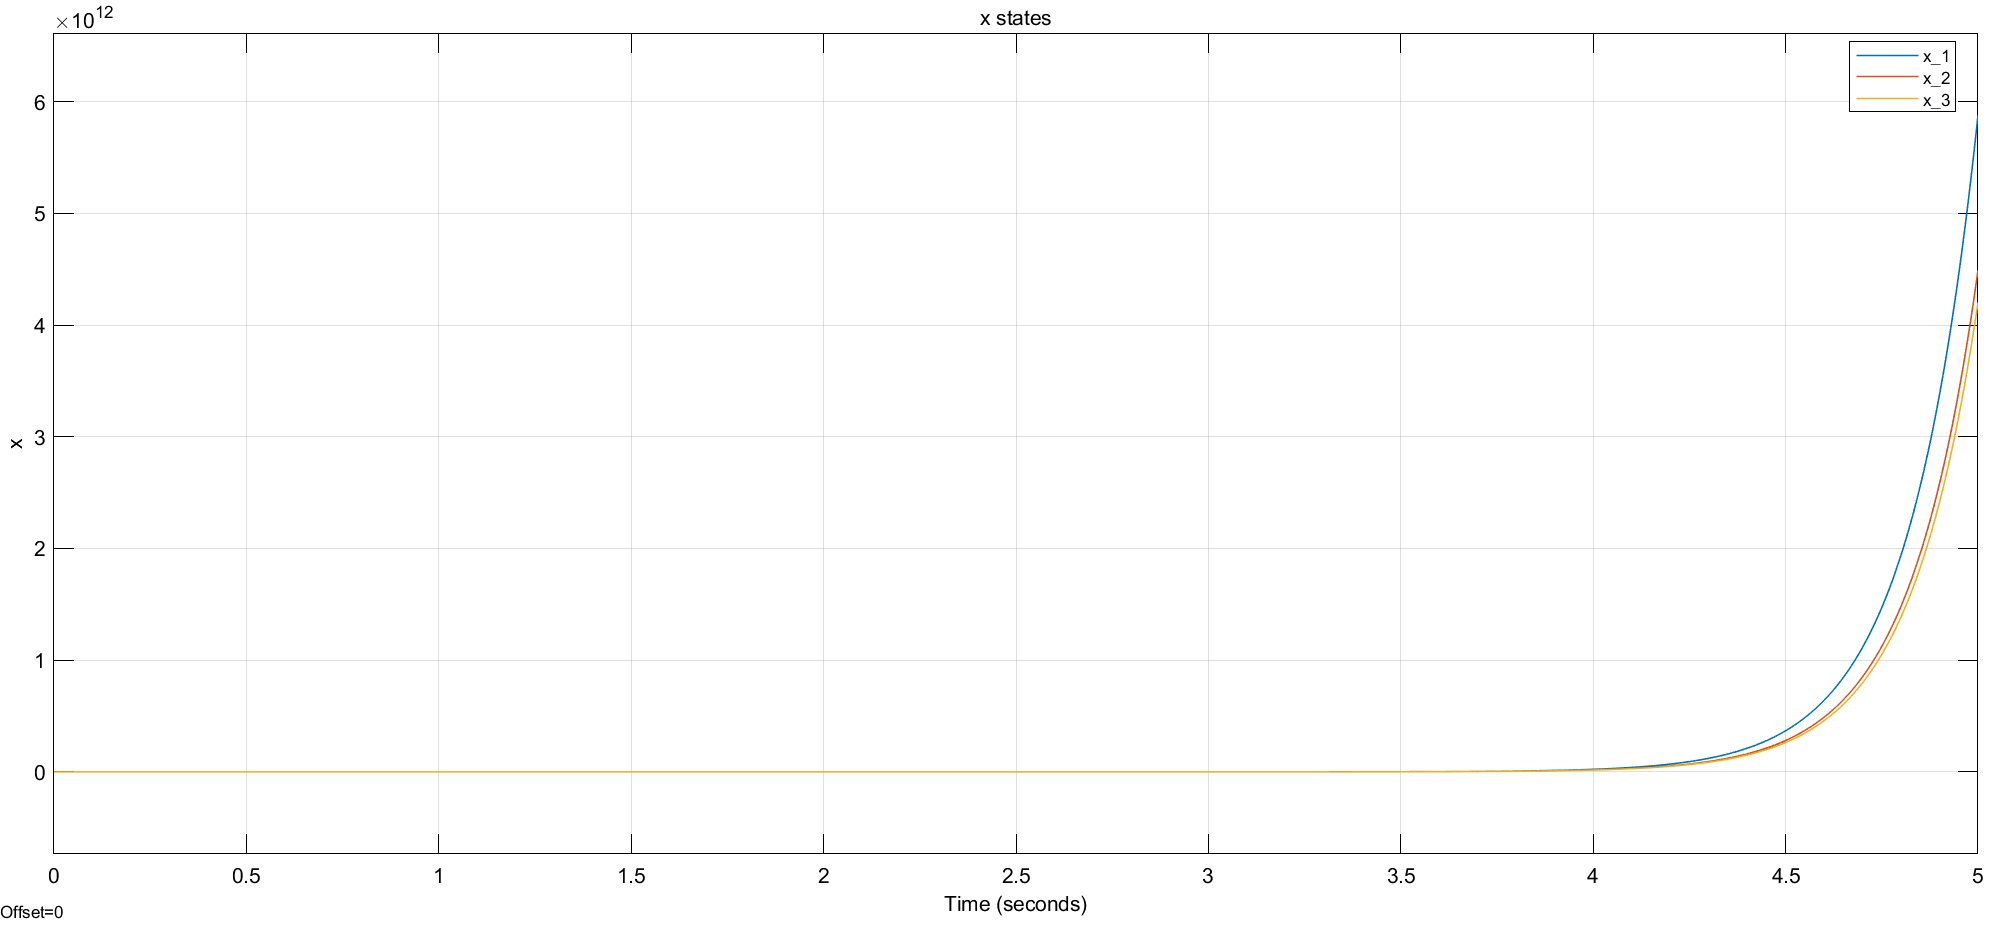
\includegraphics[width=\textwidth]{x_states}
    \caption{компоненты вектора состояний системы}
    \label{fig:x_states}
\end{figure} \\
Как можно видеть, система действительно является неустойчивой, так как все компоненты состояния стремятся в бесконечность с течением времени. \\
\ \\
Для того, чтобы система стала устойчивой можно замкнуть её регулятором $u = kx$, где $k \leq -\max_i{Re(\lambda_i)}, \ \lambda_i$ - собственные числа матрицы $A$.\\
\ \\
Итак, граничное значение параметра $k^* = -5.5410$. \\
\ \\
Система принимает следующий вид:
\[
\dot{x}=\begin{bmatrix}
-2 & 8 & 2\\
3 & -4 & 6\\
3 & 5 & -4
\end{bmatrix}x+\begin{bmatrix}
1 & 0 & 0\\
0 & 1 & 0\\
0 & 0 & 1
\end{bmatrix}kx = /k=k^*=-5.5410/ = 
\begin{bmatrix}
-7.5410 & 8 & 2\\
3 & -9.5410 & 6\\
3 & 5 & -9.5410
\end{bmatrix}x
\]\\
Собственные числа системы:
\[
\lambda_1 = 0,\ \lambda_2 = -11.8054,\ \lambda_3 = -14.8175
\]\\
Так как собственных чисел с положительной действительной частью нет и существует некратный корень (с учётом мнимой части), действительная часть которого равна нулю, то система будет находиться на так называемой \emph{границе устойчивости}, то есть компоненты состояния не сойдутся точно в 0, а сойдутся к каким-то значениям.\\
\ \\
Построим графики этой системы:
\ \\
\begin{figure}[h]
    \centering
    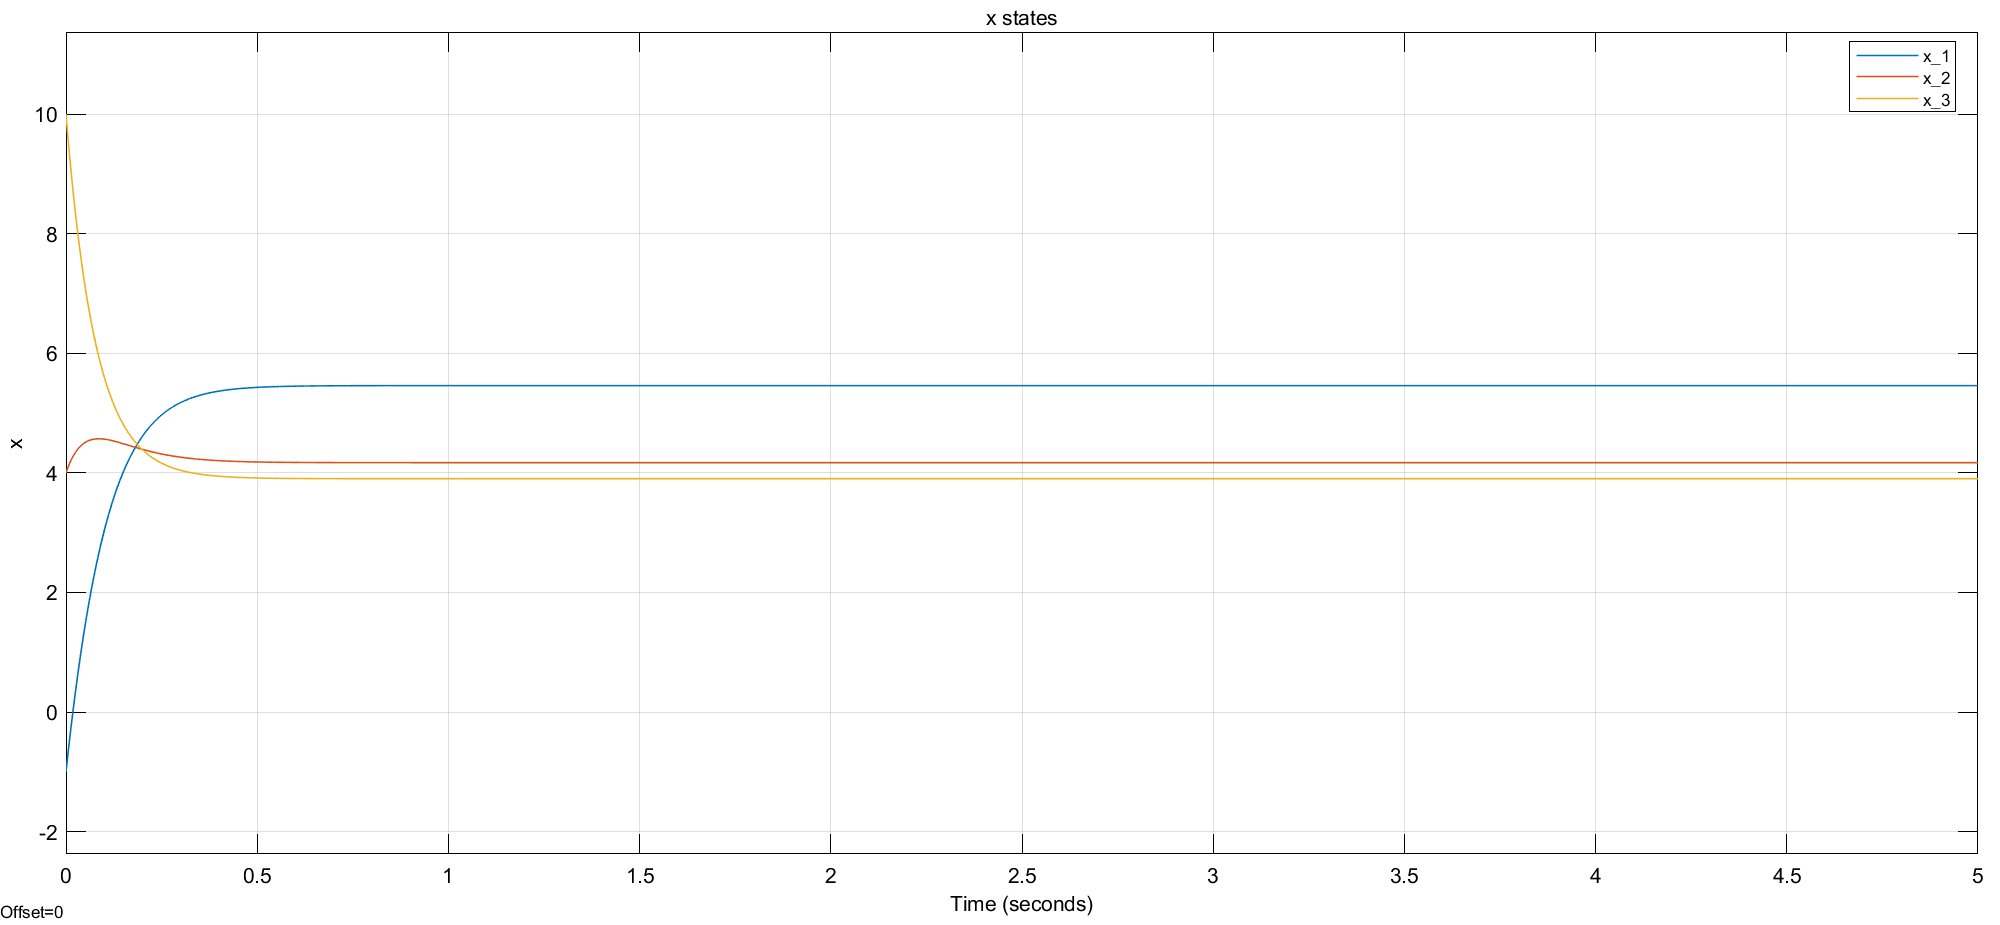
\includegraphics[width=\textwidth]{x_reg_states}
    \caption{компоненты вектора состояний замкнутой системы}
    \label{fig:x_states}
\end{figure} \\
Действительно, система уже не является неустойчивой.
\section*{Выводы}
В данной лабораторной работе были рассмотрены линейные системы в различных формах, были проведены преобразования от "вход-выход" к "вход-состояние-выход". Как убедились, данные формы представления являютя эквивалентными. \\
Также проводилось исследование системы на устойчивость с помощью анализа собственных чисел. В случае неустойчивости простой системы был найден регулятор, стабилизирующий вектор компонент. В качестве доказательств правильности расчетов были приведены графики моделирования систем из среды \emph{Simulink (Matlab)}.
\end{document}